\documentclass[11pt,a4paper]{article}

% Pacotes básicos
\usepackage[utf8]{inputenc}
\usepackage[T1]{fontenc}
\usepackage[brazil]{babel}
\usepackage{amsmath, amssymb, amsfonts, amsthm}
\usepackage{geometry}
\usepackage{graphicx}
\usepackage{xcolor}
\usepackage{hyperref}
\usepackage{fancyhdr}
\usepackage{enumitem}
\usepackage{float}
\usepackage{tikz}
\usepackage{pgfplots}
\usepackage{amsmath}
\usetikzlibrary{3d, calc}

% Layout da página
\geometry{margin=2.5cm}
\setlength{\parskip}{0.5em}
\setlength{\parindent}{0em}

% Cabeçalho e rodapé
\pagestyle{fancy}
\fancyhf{}
\rhead{Cálculo 3}
\rfoot{\thepage}

% Comandos úteis
\newcommand{\R}{\mathbb{R}}
\newcommand{\N}{\mathbb{N}}
\newcommand{\Z}{\mathbb{Z}}
\newcommand{\vect}[1]{\vec{\mathbf{#1}}}
\newcommand{\norm}[1]{\left\lVert #1 \right\rVert}

\theoremstyle{definition} % Estilo para todos (fonte romana, não itálico)
\newtheorem{theorem}{Teorema}[section]
\newtheorem{lemma}{Lema}[section]
\newtheorem{definition}{Definição}[section]
\newtheorem{example}{Exemplo}[section]
\newtheorem{remark}{Observação}[section]
\newtheorem{proposition}{Proposição}[section] % Define um ambiente "proposition"
\newenvironment{demonstracao}[1][Demonstração]{\par\noindent\textbf{#1:} }




\begin{document}

% ----- CAPA -----
\begin{titlepage}
    \centering
    \vspace*{2cm}
    {\Huge\bfseries Anotações de Cálculo 3 \par}
    \vspace{1.5cm}
    {\Large Luiz Felipe\par}
    \vfill
    {\large \today\par}
\end{titlepage}

% ----- SUMÁRIO -----
\tableofcontents
\newpage

% ----- CONTEÚDO -----
\section{Derivadas Parciais}
\subsection{Derivadas em funções de múltiplas variáveis}


\begin{definition} Dada uma função $f: \mathbb{R}^2 \to \mathbb{R}$, definimos as derivadas parciais de $f$ em relação a $x$ e $y$ da seguinte maneira:

\[
f_x(x, y) = \lim_{h \to 0} \dfrac{f(x + h,\; y) - f(x ,y)}{h}
\qquad
f_y(x, y) = \lim_{h \to 0} \dfrac{f(x,\; y + h) - f(x ,y)}{h}
\]

\end{definition}
\textbf{Interpretação geométrica das derivadas parciais}

Seja $z = f(x, y)$ representando uma superfície $S$, e considere o ponto $P(a, b, c)$ onde $c = f(a, b)$. Definimos a curva $C_1$ como a interseção de $S$ com o plano $y = b$, isto é, $C_1: z = f(x, b)$, e a curva $C_2$ como a interseção com o plano $x = a$, ou seja, $C_2: z = f(a, y)$.

As inclinações das retas tangentes às curvas $C_1$ e $C_2$ no ponto $P$ são dadas, respectivamente, por $f_x(a, b)$ e $f_y(a, b)$. Portanto, as derivadas parciais $f_x(a, b)$ e $f_y(a, b)$ podem ser interpretadas geometricamente como as inclinações das retas tangentes em $P(a, b, c)$ aos cortes $C_1$ e $C_2$ da superfície $S$ nos planos $y = b$ e $x = a$.

\begin{figure}[H]
	\centering
	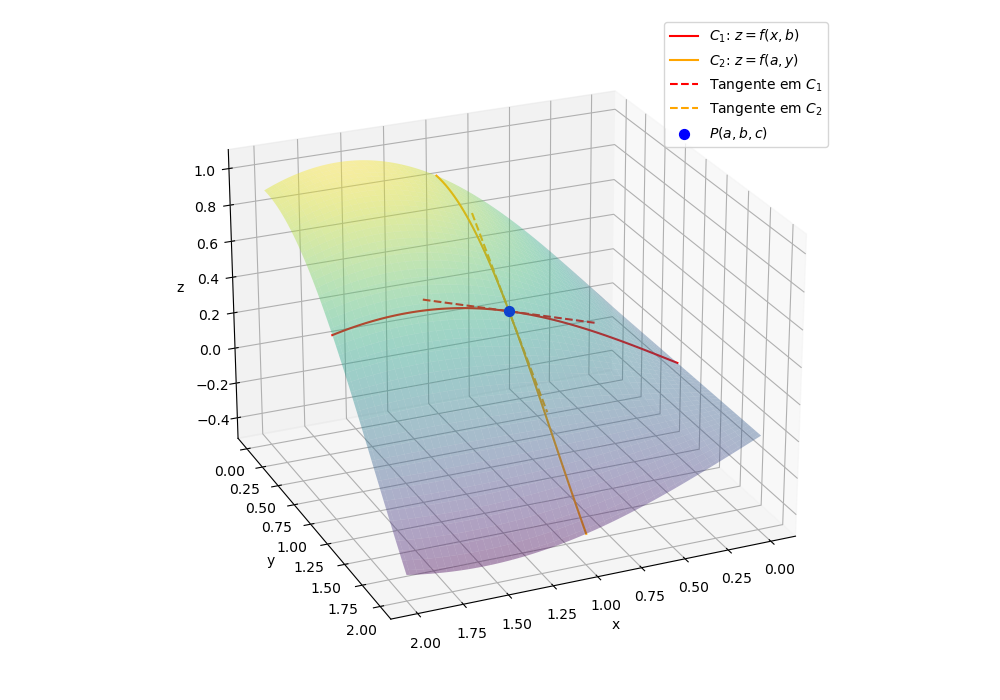
\includegraphics[width=1\linewidth]{pictures/Figure_1.png}
	\caption{Interpretação geométrica das derivadas parciais}
	\label{fig:interpretacao}
\end{figure}

\begin{definition} Dada uma função $f: \mathbb{R}^m \subset \mathbb{R}^n \to \mathbb{R}$, definimos as derivadas parciais de $f$ em relação à i-ésima variável como:

\[
\dfrac{\partial f} {\partial x_i} = \lim_{h \to 0} \dfrac{f(x_1, \dots,x_i + h , \; x_m) - f(x_1 ,\dots, x_m)}{h}
\]

\end{definition}

\begin{definition} Para derivadas parciais de ordem superior:

\[
(f_{x_i})_{x_i} = \dfrac{\partial}{\partial x_i} \left(\dfrac{\partial f} {\partial x_i} \right) = \dfrac{\partial^2f}{\partial (x_i)^2}
\]


\end{definition}

\begin{theorem}
Seja $f$ definida em uma bola aberta $D$ que contenha o ponto $(a, b)$. Se ambas as funções $f_{xy}$ e $f_{yx}$ forem contínuas em $D$, então:

\[
f_{xy}(a, b) = f_{yx}(a, b)
\]

\end{theorem}


\subsection{Planos Tangentes e Aproximações Lineares e Diferenciais}

\subsubsection{Planos Tangentes}

Suponha que uma superfície $S$ tenha a equação $z = f(x, y)$, onde $f$ tenha derivadas parciais contínuas de primeira ordem e seja $P(x_0, y_0, z_0)$ um ponto na superfície S. pegue as curvas $C_1$ e $C_2$ que são respectivamente $f_x(x, y_0)$ e $f_y(x_0, y)$ seja $T_1, T_2$ retas tangentes as curvas $C_1, C_2$ obtemos um \textbf{Plano Tangente} a superfície $S$ no ponto $P$. 


\begin{figure}[H]
	\centering
	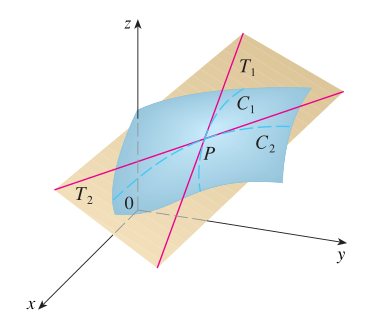
\includegraphics[width=0.4\linewidth]{pictures/plano.png}
	\label{fig:interpretacao}
	\caption{Plano Tangente Ao Ponto P}
\end{figure}

Temos que a equação do plano passando por $P(x_0, y_0, z_0)$ tem a forma: 

\begin{equation}
	A(x - x_0) + B(y - y_0) + C(z - z_0) = 0
	\label{equacao_plano_1}
\end{equation}

Dividindo em ambos os lados por -C temos 

\begin{equation}
	\dfrac{A}{-C}(x - x_0) + \dfrac{B}{-C}(y - y_0) + -z + z_0 = 0
	\label{equacao_plano_2}
\end{equation}

Escrevendo $a = -\dfrac{A}{C}$ e $b = -\dfrac{B}{C}$ temos 


\begin{equation}
	a(x - x_0) + b(y - y_0) = z - z_0 
	\label{equacao_plano_3}
\end{equation}

Repare que quando $y = y_0$ obtemos a seguinte equação 

\begin{equation}
	a(x - x_0) + b(y - y_0) = z - z_0 
	\label{equacao_plano_4}
\end{equation}

Se a equação \ref{equacao_plano_1} representa o plano temos que a equação \ref{equacao_plano_4} representa a reta $T_1$ logo sua inclinação é $a = f_x(x_0, y_0)$. 

De maneira análoga quando $x = x_0$ obtemos a seguinte equação:

\begin{equation}
	b(y - y_0) = z - z_0 
	\label{equacao_plano_5}
\end{equation}

Temos que a equação \ref{equacao_plano_5} representa a reta $T_2$ portanto sua inclinação é $b = f_y(x_0, y_0)$ o que motiva a seguinte definição 

\begin{definition} Sendo $f: \R^2 \rightarrow \R$ uma função onde suas derivadas parciais são contínuas uma equação do plano tangente a superfície $z = f(x, y)$ no ponto $P(x_0, y_0, z_0)$ é dada por 

\[
	z - z_0 = f_x(x_0, y_0)(x - x_0) + f_y(x_0, y_0)(y - y_0) 
\]
\end{definition}

\subsubsection{Aproximações Lineares}

Sabemos que a equação do plano do plano tangente ao gráfico de uma função $f$ cujas derivadas parciais são contínuas no ponto $(a, b, f(a, b))$ é 

\[
z = f(a, b) + f_x(a, b)(x - a) + f_y(a, b)(y - b) 
\]

Temos que a função linear cujo gráfico é esse plano tangente é 

\[
	L(x, y) = f(a, b) + f_x(a, b)(x - a) + f_y(a, b)(y - b) 
\]

Denominamos de \textbf{linearização} de $f$ em $(a, b)$ a aproximação: 

\[
	f(x, y) \approx f(a, b) + f_x(a, b)(x - a) + f_y(a, b)(y - b) 
\]

ou seja obtemos boas aproximações da função original através de $L(x,y)$ porém elas só ficam precisas em torno de $(a, b)$. o que motiva a seguinte definição 

\begin{definition} Sendo $f: \R^2 \rightarrow \R$ uma função onde suas derivadas parciais são contínuas temos que a aproximação em $(a, b)$ é dada da seguinte maneira 

\[
f(x, y) \approx f(a, b) + f_x(a, b)(x - a) + f_y(a, b)(y - b) 
\]

\end{definition}
%% adicionar dois exemplos com graficos no matplotlib 


\subsubsection{Diferenciais}

\paragraph{Uma variável.}
Seja $f:\mathbb{R}\to\mathbb{R}$ e fixe $x_0\in\mathbb{R}$. Dizemos que $f$ é derivável em $x_0$ se existe $f'(x_0)$ tal que, para $\Delta x\to 0$,
\[
\Delta y \;=\; f(x_0+\Delta x)-f(x_0) \;=\; f'(x_0)\,\Delta x \;+\; r(\Delta x),
\qquad \text{com } \frac{r(\Delta x)}{|\Delta x|}\longrightarrow 0.
\]
De forma equivalente (versão $\varepsilon$–$\delta$): 
\[
\forall\,\varepsilon>0\;\exists\,\delta>0\;\text{ tal que }\;|\Delta x|<\delta \;\Rightarrow\; 
\bigl|\Delta y - f'(x_0)\Delta x\bigr|\le \varepsilon\,|\Delta x|.
\]
O \emph{diferencial} de $f$ em $x_0$ é a aplicação linear dada por
\[
dy \;=\; f'(x_0)\,dx,
\]
onde $dx$ é um incremento independente. Assim, para $dx$ pequeno,
\[
f(x_0+dx) \;\approx\; f(x_0) + dy \;=\; f(x_0) + f'(x_0)\,dx.
\]

\paragraph{Duas variáveis.}
Seja $f:\mathbb{R}^2\to\mathbb{R}$ e fixe $(x_0,y_0)$. Dizemos que $f$ é \emph{diferenciável} em $(x_0,y_0)$ se existe uma aplicação linear 
\[
L(\Delta x,\Delta y)=a\,\Delta x + b\,\Delta y
\]
tal que, para $h=(\Delta x,\Delta y)\to(0,0)$,
\[
\Delta z \;=\; f(x_0+\Delta x,y_0+\Delta y) - f(x_0,y_0)
\;=\; L(\Delta x,\Delta y) \;+\; r(\Delta x,\Delta y),
\qquad \text{com } \frac{|r(\Delta x,\Delta y)|}{\sqrt{(\Delta x)^2+(\Delta y)^2}}\longrightarrow 0.
\]
Nessa situação, $a=f_x(x_0,y_0)$ e $b=f_y(x_0,y_0)$, de modo que o \emph{diferencial total} em $(x_0,y_0)$ é
\[
dz \;=\; f_x(x_0,y_0)\,dx \;+\; f_y(x_0,y_0)\,dy,
\]
e vale a aproximação de primeira ordem
\[
\Delta z \;=\; dz \;+\; o\!\left(\sqrt{(\Delta x)^2+(\Delta y)^2}\right).
\]
De forma equivalente (versão $\varepsilon$–$\delta$):
\[
\forall\,\varepsilon>0\;\exists\,\delta>0\;\text{ se }\sqrt{(\Delta x)^2+(\Delta y)^2}<\delta \;\Rightarrow\;
\left|\Delta z - \bigl(f_x(x_0,y_0)\Delta x + f_y(x_0,y_0)\Delta y\bigr)\right|
\le \varepsilon\,\sqrt{(\Delta x)^2+(\Delta y)^2}.
\]

\begin{definition}
	Seja $f:\mathbb{R}^2\to\mathbb{R}$. Diz-se que $f$ é \emph{diferenciável} em $(x_0,y_0)$ se existem números reais $a,b$ e uma função $r(\Delta x,\Delta y)$ tais que
	\[
	\Delta z \;=\; a\,\Delta x + b\,\Delta y \;+\; r(\Delta x,\Delta y),
	\qquad
	\frac{|r(\Delta x,\Delta y)|}{\sqrt{(\Delta x)^2+(\Delta y)^2}}\longrightarrow 0
	\quad\text{quando }(\Delta x,\Delta y)\to(0,0).
	\]
	Nesse caso, $a=f_x(x_0,y_0)$ e $b=f_y(x_0,y_0)$, e o diferencial total é $dz=f_x(x_0,y_0)\,dx+f_y(x_0,y_0)\,dy$.
\end{definition}

\begin{remark}
	(i) $dz$ é a parte \emph{linear} do incremento real $\Delta z$; por isso, em geral $\Delta z\neq dz$, mas $\Delta z - dz = o(\|( \Delta x,\Delta y)\|)$. 
	(ii) A mera existência das derivadas parciais não garante diferenciabilidade; um critério suficiente é a continuidade de $f_x$ e $f_y$ em uma vizinhança de $(x_0,y_0)$.
\end{remark}

\subsection{Regra Da Cadeia e Derivação implícita}

\begin{theorem}
	Supondo que $z = f(x, y)$ seja uma função diferenciável, onde $x = g(t)$ e $y = h(t)$ são funções diferenciáveis de $t$, então $z$ é uma função diferenciável de $t$, e segue que
	
	\[
	\dfrac{dz}{dt} = \dfrac{\partial f}{\partial x} \dfrac{dx}{dt} + \dfrac{\partial f}{\partial y} \dfrac{dy}{dt}
	\]
\end{theorem}

\begin{proof}
	Seja $z = f(x, y)$ uma função diferenciável, com $x = g(t)$ e $y = h(t)$ funções diferenciáveis de $t$. Então, ao variar $t$ em uma pequena quantidade $\Delta t$, temos variações $\Delta x$ em $x$ e $\Delta y$ em $y$, que por sua vez causam uma variação $\Delta z$ em $z$.
	
	Como $f$ é diferenciável, temos que a variação $\Delta z$ pode ser aproximada por:
	
	\[
	\Delta z \approx \frac{\partial f}{\partial x} \Delta x + \frac{\partial f}{\partial y} \Delta y
	\]
	
	Dividindo ambos os lados por $\Delta t$, obtemos:
	
	\[
	\frac{\Delta z}{\Delta t} \approx \frac{\partial f}{\partial x} \frac{\Delta x}{\Delta t} + \frac{\partial f}{\partial y} \frac{\Delta y}{\Delta t}
	\]
	
	Tomando o limite quando $\Delta t \to 0$, e usando a continuidade e a diferenciabilidade de $x(t)$ e $y(t)$, obtemos:
	
	\[
	\frac{dz}{dt} = \frac{\partial f}{\partial x} \frac{dx}{dt} + \frac{\partial f}{\partial y} \frac{dy}{dt}
	\]
	
	Portanto, a derivada de $z$ em relação a $t$ é dada pela fórmula da Regra da Cadeia.
\end{proof}

\begin{definition}[Regra da Cadeia — Caso 2]
	Suponha que $z = f(x, y)$ seja uma função diferenciável de $x$ e $y$, onde $x = g(s, t)$ e $y = h(s, t)$ são funções diferenciáveis de $s$ e $t$.
	
	Então, $z$ é uma função diferenciável de $s$ e $t$, e temos:
	
	\[
	\frac{\partial z}{\partial s} = \frac{\partial f}{\partial x} \frac{\partial x}{\partial s} + \frac{\partial f}{\partial y} \frac{\partial y}{\partial s}
	\quad \text{e} \quad
	\frac{\partial z}{\partial t} = \frac{\partial f}{\partial x} \frac{\partial x}{\partial t} + \frac{\partial f}{\partial y} \frac{\partial y}{\partial t}
	\]
\end{definition}

\begin{theorem}
	Suponha que $u$ seja uma função diferenciável de $n$ variáveis $x_1, x_2, \dots, x_n$, onde cada $x_j$ é uma função diferenciável de $m$ variáveis $t_1, t_2, \dots, t_m$. Então $u$ é uma função diferenciável de $t_1, t_2, \dots, t_m$ e, para cada $i = 1, 2, \dots, m$, temos:
	
	\[
	\frac{\partial u}{\partial t_i} 
	= 
	\frac{\partial u}{\partial x_1} \frac{\partial x_1}{\partial t_i}
	+ \frac{\partial u}{\partial x_2} \frac{\partial x_2}{\partial t_i}
	+ \dots 
	+ \frac{\partial u}{\partial x_n} \frac{\partial x_n}{\partial t_i}
	\]
	
	ou, de forma compacta:
	
	\[
	\frac{\partial u}{\partial t_i} 
	= 
	\sum_{j=1}^{n} \frac{\partial u}{\partial x_j} \frac{\partial x_j}{\partial t_i}
	\]
\end{theorem}

\end{document}
